\section{Class 使用方法}

\begin{table}[H]
	\begin{center}
{\fontsize{10pt}{12}\selectfont\ttfamily
\begin{tabular}{|c|p{70mm}|p{75mm}|}
 \hline%
{序 號} & {入 例} & {說 明} \\ \hline %
0 & \verb+\documentclass[pdfm,b5paper]{sz}+ & 小川原版class改,字號不嚴格對應標準字號。\\
1 & \verb+\documentclass[pdfm,b5paper]{sz9}+ & 正文 9 pt 系列,按此實際字號換算class字號。\\
2 & \verb+\documentclass[pdfm,b5paper]{sz10}+ & 正文 10 pt 系列(同上)。\\
3 & \verb+\documentclass[pdfm,b5paper]{sz11}+ & 正文 11 pt 系列(同上)。\\
4 & \verb+\documentclass[pdfm,b5paper]{sz12}+ & 正文 12 pt 系列(同上)。\\
5 & \verb+\documentclass[pdfm,b5paper]{sz10x}+ & 正文 五號(10.5pb 合 10.53937 pt)系列。\\
\hline%
\end{tabular} }
	\end{center}
\end{table}

\section{小川 弘和 SZ.CLS 字號對照表}\label{sec:intro}

\subsection{正文 9 pt 系列}
\begin{figure}[H]
\begin{center}
\caption{小川原版class改(sz.cls)}
{ 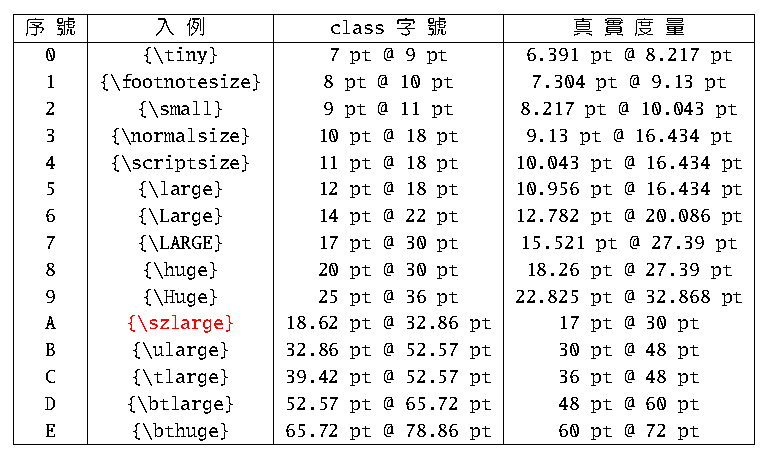
\includegraphics[scale=1]{figures/sz.pdf}}
\end{center}
\par 正文 9 pt 系列,字號不嚴格對應標準字號。
\end{figure}

\begin{figure}[H]
\begin{center}
\caption{正文 9 pt 系列(sz9.cls)}
{ 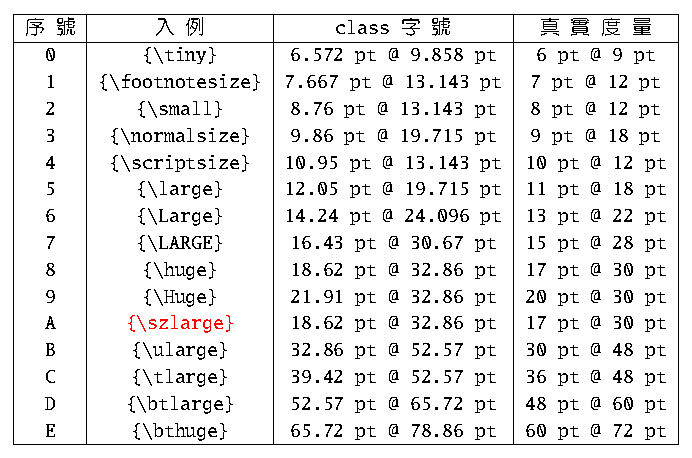
\includegraphics[scale=1]{figures/sz9.pdf}}
\end{center}
\par 正文 9 pt 系列,按此實際字號換算class字號。
\end{figure}

\subsection{正文 10 pt 系列}
\begin{figure}[H]
\begin{center}
\caption{正文 10 pt 系列(sz10.cls)}
{ 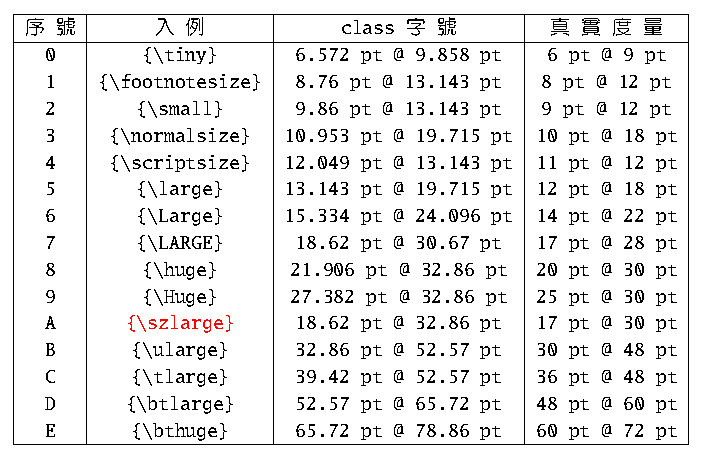
\includegraphics[scale=1]{figures/sz10.pdf}}
\end{center}
\par 正文 10 pt 系列,按此實際字號換算class字號。
\end{figure}

\subsection{正文 11 pt 系列}
\begin{figure}[H]
\begin{center}
\caption{正文 11 pt 系列(sz11.cls)}
{ 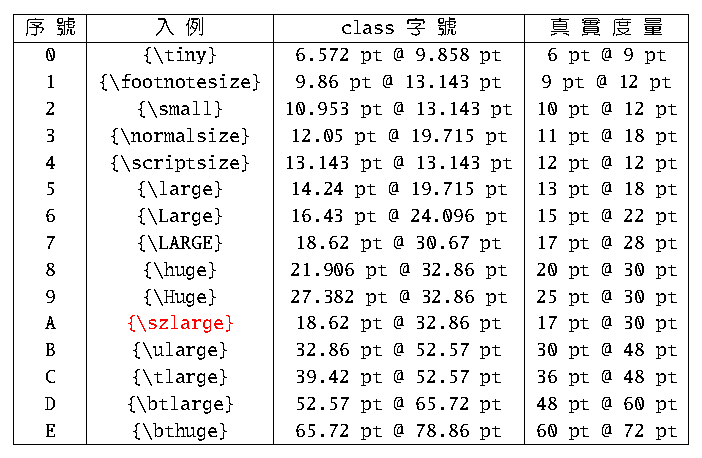
\includegraphics[scale=1]{figures/sz11.pdf}}
\end{center}
\par 正文 11 pt 系列,按此實際字號換算class字號。
\end{figure}


\subsection{正文 12 pt 系列}
\begin{figure}[H]
\begin{center}
\caption{正文 12 pt 系列(sz12.cls)}
{ 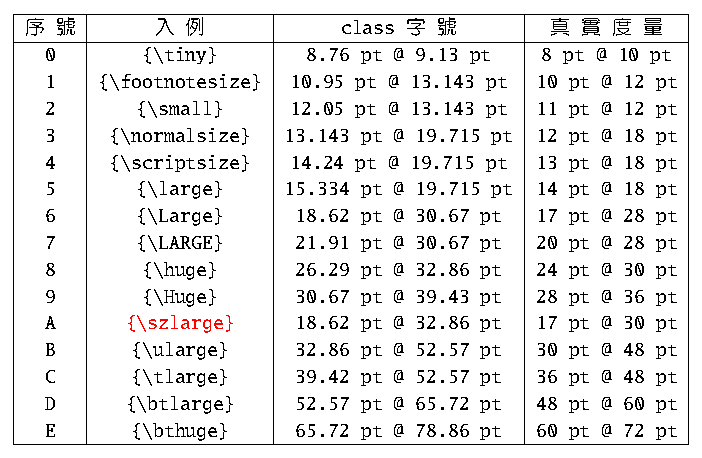
\includegraphics[scale=1]{figures/sz12.pdf}}
\end{center}
\par 正文 12 pt 系列,按此實際字號換算class字號。
\end{figure}

\subsection{正文 五號 系列}
\begin{figure}[H]
\begin{center}
\caption{正文 五號 系列(sz10x.cls)}
{ 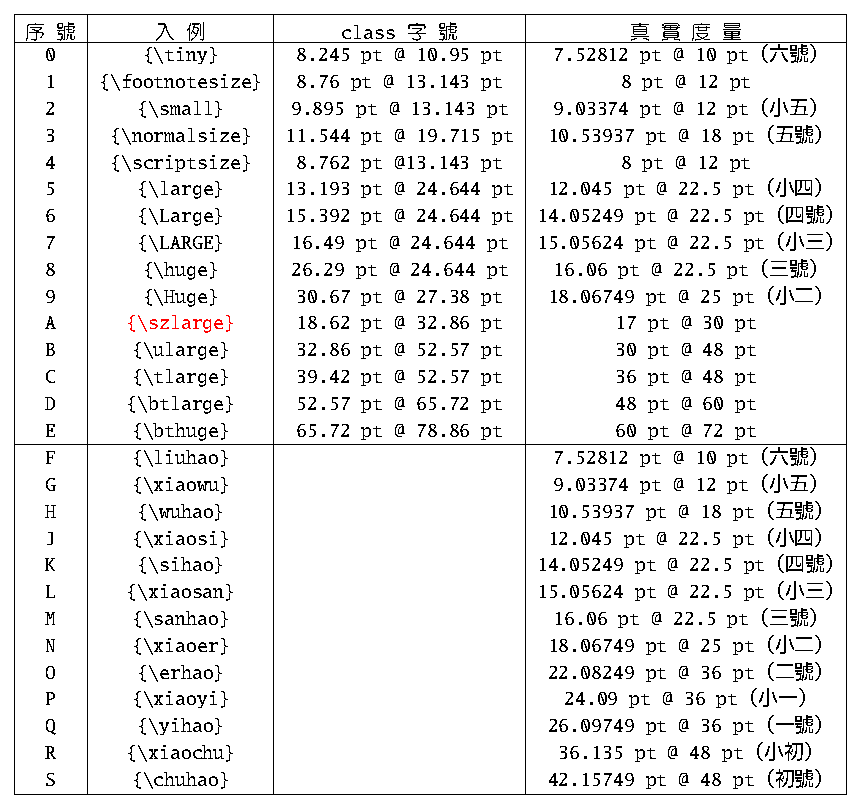
\includegraphics[scale=1]{figures/sz10x.pdf}}
\end{center}
\par 正文  五號  系列,按此實際字號換算class字號。
\end{figure}



\section{up{\LaTeX}常用命令舉例}

\begin{itemize}
\item{}{\verb+\yato+}和{\verb+\tate+}:这两个命令是让你确定横排还是竖排。实际上还有一个{\verb+\dtou+}命令,也是竖排,但是是从下到上,这个命令只有在一些开发文档上才能看到。
\item{}{\verb+\jfont+}和{\verb+\tfont+}:这两个命令和TeX原始的{\verb+\font+}命令一样,但是分别指定的是横排和竖排的字体。在{p\LaTeX}扩展的NFSS编码中,横排和竖排的字体编码为JY1和JT1,{up\LaTeX}中相应的编码为JY2和JT2,{Lua\TeX}-ja中对应的编码为JY3和JT3。
\item{}{\verb+\jfam+}:这个命令是用来定义字体族的,请参考{\TeX}中的{\verb+\fam+}用法。
\item{}{\verb+zh+}和{\verb+zw+}:这两个是相对单位,类似于tfm中定义的ex和em,指的是一个汉字的高度和宽度,定义来源于jfm中的相关部分。
\item{}{\verb+\ybaselineshift+}和{\verb+\tbaselineshift+}:这两个命令是用来对齐汉字和西文之间的基线的,通常情况下都需要进行调整,让汉字与西文对齐。
\item{}{\verb+\kanjiskip+}和{\verb+\xkanjiskip+}:两个命令分别对应的是:汉字-汉字之间距离,汉字-西文距离。 有点像{\TeX}中{\verb+\spaceskip+}(此命令只對西文起作用)。
\item{}{\verb+\kansuji+}和{\verb+\kansujichar+}:前者将阿拉伯数字转换成汉字,如{\verb+\kansuji12+}转换成“一二”。后者给数字指定汉字,如{\verb+\kansujichar1=`壱+}。
\item{}{\verb+\euc+}、{\verb+\jis+}和{\verb+\sjis+}:这个命令相当于{\verb+\char+},就是限定了编码。
\item{}{\verb+\prebreakpenalty+}和{\verb+\postbreakpenalty+}:这两个命令分别在某个字符前或者字符后添加penalty,以达到避头尾的效果。如{\verb+\prebreakpenalty`あ=1000+}。
\item{}{\verb+\jcharwidowpenalty+}:这是控制孤行的。
\item{}{\verb+\xspcode+}:控制{\verb+\xkanjiskip+}插入的命令,对象是西文字符,如{\verb+\xspcode`A=0+}。可选的值为:0,1,2,3。0的情况:禁止在左侧插入。1的情况:允许在左侧插入。2的情况:允许在右侧插入。3的情况:允许两侧插入。
\item{}{\verb+\inhibitglue+}:禁止glue插入。
\item{}{\verb+\autospacing+}和{\verb+\noautospacing+}:允许/禁止汉字-汉字之间插入glue。
\item{}{\verb+\autoxspacing+}和{\verb+\noautoxspacing+}:允许/禁止汉字-西文之间插入glue。
\item{}{\verb+\inhibitxspcode+}:和{\verb+\xspcode+}类似,但是这个命令对象是汉字字符。
\item{}{\verb+\kcatcode+}:类似于TeX的{\verb+\catcode+}。
\end{itemize}

\par\href{https://www.zhihu.com/question/20544732/answer/15437234}%
{詳見``如何使用 LaTeX 輸出豎版排版的文章或書籍?"}


%\clearpage

\section{為up{\LaTeX}配置本地字體}

\subsection{字體實現的三種思路。}
\par\noindent
思路一:通過NFSS設置方法,將已有的tfm及同名vf映射到本地字體。\\
優點:簡單方便,不產生新的vf和tfm,僅適用於臨時占用。\\
缺點:會占用系統預設的tfm和vf。\\[5mm]
思路二:使用PXcopyfont工具包為本地字體複製配套的tfm和vf。\\
優點:為每一個本地字體都配置單獨的vf及tfm,可以避免同系統自帶的tfm及vf撞車;\\
\hspace{3zw}便於移植到下一台計算機。\\
缺點:占用硬盤資源大。配置難度大。\\[5mm]
思路三:使用Jfmutil工具包為本地字體創建全新的tfm和vf。\\
優點:可以自定義禁則。便於移植到下一台計算機。\\
缺點:配置難度太大,禁則編寫難度太高,往往不容易成功。


\subsection{簡體中文字體宏包}
\par
使用\verb+ctex+宏包可以调用Windows/OS X/Linux 本地字体。
使用此package前請先閲讀ctex.pdf 手冊,目前中文繁體支持仍然很差,
除楷體和宋體外,隸書僅支持簡體中文使用。
\begin{lstlisting}[firstnumber=1]
\usepackage[fontset=windows]{ctex}
%\usepackage[fontset=adobe]{ctex}
\end{lstlisting}


\subsection{{up\LaTeXe}字體設置方法(NFSS)}

\par{}使用 八登崇之 PXcopyfont 工具包。(見附件 PXcopyfont 文件夾。)
\par{}安裝 perl 工具包。Windows 10 系統可以下載使用 {ActivePerl}。

\subsubsection*{案例一創建 {kleePro} 虛擬字體和TFM文件}

(請勿照抄此案例。)

\par{}{\bfseries{Windows系統}}在記事本中寫入以下語句,另存為 \uwave{\red{MK KLEE.BAT}}。
\begin{lstlisting}[firstnumber=1]
perl pxcopyfont.pl -o upjisr-h klee-m-jy2 r-klee-m-jy2 r-klee-m-jy2x
perl pxcopyfont.pl -o upjisr-v klee-m-jt2 r-klee-m-jt2
perl pxcopyfont.pl -o jis klee-m-jy1 r-klee-m-jy1
perl pxcopyfont.pl -o jis-v klee-m-jt1 r-klee-m-jt1
perl pxcopyfont.pl -o upjisr-h klee-db-jy2 r-klee-db-jy2 r-klee-db-jy2x
perl pxcopyfont.pl -o upjisr-v klee-db-jt2 r-klee-db-jt2
perl pxcopyfont.pl -o jis klee-db-jy1 r-klee-db-jy1
perl pxcopyfont.pl -o jis-v klee-db-jt1 r-klee-db-jt1
\end{lstlisting}

\par{}保存後,直接雙擊執行。不能用管理員權限,否則進入system32系統文件夾下了。
\par{}現在打開
{\color{red}C:$\backslash$texlive$\backslash$texmf-local$\backslash$fonts$\backslash$vf},
新建klee文件夾,將vf字體複製進去。
\par{}打開
{\color{red}C:$\backslash$texlive$\backslash$texmf-local$\backslash$fonts$\backslash$tfm},
新建klee文件夾,將tfm文件複製進去。
\par{}執行\red{mktexlsr}刷新{\TeX}文件樹。


\subsubsection*{案例二創建 {kleePro} 配置文件}

(請勿照抄此案例。)

\par{}參考{doratex}的博客,在{mysample.tex}中寫入以下語句,使用
{\color{red}\verb+{ptex2pdf -l -u  mysample}+}
進行編譯:
\begin{lstlisting}[firstnumber=1]
%#!使用uplatex 編譯
\documentclass[uplatex]{jsarticle}
\usepackage{plext}% 縦組用
\pagestyle{empty}
%%% klee ファミリーに m と db のシリーズを定義
\DeclareFontFamily{JY2}{klee}{}
\DeclareFontFamily{JT2}{klee}{}

\DeclareFontShape{JY2}{klee}{m}{n}{<->s*[0.924690]klee-m-jy2}{}
\DeclareFontShape{JY2}{klee}{m}{it}{<->ssub*klee/m/n}{}
\DeclareFontShape{JY2}{klee}{m}{sl}{<->ssub*klee/m/n}{}
\DeclareFontShape{JY2}{klee}{m}{sc}{<->ssub*klee/m/n}{}
\DeclareFontShape{JT2}{klee}{m}{n}{<->s*[0.924690]klee-m-jt2}{}
\DeclareFontShape{JT2}{klee}{m}{it}{<->ssub*klee/m/n}{}
\DeclareFontShape{JT2}{klee}{m}{sl}{<->ssub*klee/m/n}{}
\DeclareFontShape{JT2}{klee}{m}{sc}{<->ssub*klee/m/n}{}

\DeclareFontShape{JY2}{klee}{db}{n}{<->s*[0.924690]klee-db-jy2}{}
\DeclareFontShape{JY2}{klee}{db}{it}{<->ssub*klee/db/n}{}
\DeclareFontShape{JY2}{klee}{db}{sl}{<->ssub*klee/db/n}{}
\DeclareFontShape{JY2}{klee}{db}{sc}{<->ssub*klee/db/n}{}
\DeclareFontShape{JT2}{klee}{db}{n}{<->s*[0.924690]klee-db-jt2}{}
\DeclareFontShape{JT2}{klee}{db}{it}{<->ssub*klee/db/n}{}
\DeclareFontShape{JT2}{klee}{db}{sl}{<->ssub*klee/db/n}{}
\DeclareFontShape{JT2}{klee}{db}{sc}{<->ssub*klee/db/n}{}

\DeclareRobustCommand\kleem{\kanjifamily{klee}\kanjiseries{m}\selectfont}
\DeclareRobustCommand\kleedb{\kanjifamily{klee}\kanjiseries{db}\selectfont}

% dvipdfmx special の発行
\AtBeginDvi{%
  \special{pdf:mapline klee-m-jy2    UniJIS2004-UTF16-H FOT-KleePro-M.otf}%
  \special{pdf:mapline klee-m-jt2    UniJIS2004-UTF16-V FOT-KleePro-M.otf}%
  \special{pdf:mapline klee-db-jy2   UniJIS2004-UTF16-H FOT-KleePro-DB.otf}%
  \special{pdf:mapline klee-db-jt2   UniJIS2004-UTF16-V FOT-KleePro-DB.otf}%
}

\begin{document}
\parbox<y>{22zw}{%
{\kleem{}(*クレーミディアムの横組サンプル、「約物の“テスト”」。*)}\par
{\kleedb{}(*クレーデミボールドの横組サンプル、「約物の“テスト”」。*)}}
\vspace{5mm}
\parbox<t>{12zw}{%
{\kleem{}(*クレーミディアムの縦組サンプル、「約物の〝テスト?」。*)}\par
{\kleedb{}(*クレーデミボールドの縦組サンプル、「約物の〝テスト?」。*)}}
\end{document}
\end{lstlisting}

\begin{figure}[H]
\par\quad\marg{出力例:}
\begin{center}
\fbox{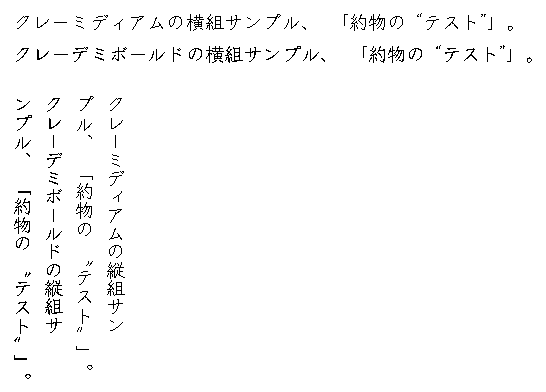
\includegraphics[width=0.6\textwidth]{figures/06.pdf}}
\end{center}
\end{figure}

%\clearpage
\subsection{簡體中文本地字體}

\par{}參照前文
配置虛擬字體和tfm。然後指定mapline為{UniGB-UTF16-H}和{UniGB-UTF16-V},
或者{UniGB-UCS2-H}和{UniGB-UCS2-V}。 或者使用 {unicode}作爲{mapline}。
示例如下:

\begin{lstlisting}[firstnumber=1]
  \special{pdf:mapline fzks-m-jy2   unicode  FZKSGBXS10.ttf}% 方正楷書 (*GB18030-S10*)版
  \special{pdf:mapline fzks-m-jt2   unicode  FZKSGBXS10.ttf -w 1}% -w 1 表示垂直排版模式
  \special{pdf:mapline fzks-sip-m-jy2   unicode  FZKaiS(SIP).TTF}%方正楷書(*S-SIP(CJK-B版)*)
  \special{pdf:mapline fzks-sip-m-jt2   unicode  FZKaiS(SIP).TTF -w 1}%
  \special{pdf:mapline fzxss-m-jy2   UniGB-UTF16-H  FZXSSGBX.TTF}% 方正新書宋 GB18030
  \special{pdf:mapline fzxss-m-jt2   UniGB-UTF16-V  FZXSSGBX.TTF}%
\end{lstlisting}

\subsection{使用{Pxchfon}宏包配置日文版思源字體}
\par{}在{mysample.tex}中寫入以下語句:

\begin{lstlisting}[firstnumber=1]
\usepackage[uplatex,deluxe]{otf}               % 多字重支持
%\usepackage[sourcehan]{pxchfon}                 % 不使用 JIS2004 字形
\usepackage[sourcehan,prefer2004jis]{pxchfon}    %   使用 JIS2004 字形

\setminchofont{SourceHanSerif-Medium.otf}
\setlightminchofont{SourceHanSerif-Regular.otf}
\setboldminchofont{SourceHanSerif-Bold.otf}
\setgothicfont{SourceHanSans-Medium.otf}
\setmediumgothicfont{SourceHanSans-Regular.otf}
\setboldgothicfont{SourceHanSans-Bold.otf}
\setxboldgothicfont{SourceHanSans-Heavy.otf}
\setmarugothicfont{SourceHanSans-Regular.otf}
\end{lstlisting}

(行5 - 12 是 sourcehan 選項時預設的,與之等價,詳見 pxchfon.pdf)

\begin{table}[H]
\begin{center}
\caption{pxchfon 等價命令}
{\fontsize{8pt}{12}\selectfont\ttfamily
\begin{tabular}{|l|l|l|}
 \hline
 OTF/TTF 命令 & TTC 命令 & 用途 \\ \hline
$\backslash$setminchofont\{*.otf/*.ttf\} & $\backslash$setminchofont[番號]\{*.ttc\} & 設置正文明朝體;\\
$\backslash$setlightminchofont\{*.otf/*.ttf\} & $\backslash$setlightminchofont[番號]\{*.ttc\} & 設置細明朝體;\\
$\backslash$setboldminchofont\{*.otf/*.ttf\} & $\backslash$setboldminchofont[番號]\{*.ttc\} & 設置粗明朝體;\\
$\backslash$setgothicfont\{*.otf/*.ttf\} & $\backslash$setgothicfont[番號]\{*.ttc\} & 設置哥特體(細黑體);\\
$\backslash$setmediumgothicfont\{*.otf/*.ttf\} & $\backslash$setmediumgothicfont[番號]\{*.ttc\} & 設置中等哥特體;\\
$\backslash$setboldgothicfont\{*.otf/*.ttf\} & $\backslash$setboldgothicfont[番號]\{*.ttc\} & 設置粗哥特體;\\
$\backslash$setxboldgothicfont\{*.otf/*.ttf\} & $\backslash$setxboldgothicfont[番號]\{*.ttc\} & 設置特粗哥特體;\\
$\backslash$setmarugothicfont\{*.otf/*.ttf\} & $\backslash$setmarugothicfont[番號]\{*.ttc\} & 設置丸書體(即圓體)。\\ \hline
\end{tabular} }
\end{center}
\end{table}


\subsection{東亞字體CMAP簡介}
\par{}CMAP是對字符映射起到索引作用的文件。(見表3)

\subsection{CID-Key和CID符號}

\par{}{up\LaTeXe}自帶一些系統命令,可以調用系統字體(如小塚明朝 kozuka-pr6n)的CID字和符號。
具體CID編號需檢索技術文檔{5078.Adobe-Japan1-6.pdf},網頁搜索即可獲取。相關示例(見表4)


\begin{table}[H]
\caption{東亞字體CMAP簡介}
{\fontsize{8pt}{12}\selectfont\ttfamily
\begin{tabular}{|c|l|l|c|l|}
\hline
 \multicolumn{1}{|c|}{言 語} & \multicolumn{1}{|c|}{CMAP(橫)}%
  &\multicolumn{1}{|c|}{CMAP(縱)}& \multicolumn{1}{|c|}{工具引擎} & \multicolumn{1}{|c|}{備注} \\ \hline
日本語& 2004-H & 2004-V & {p\LaTeX}、{p\TeX} & 適用於JIS2004字形 \\
日本語& UniJIS-UTF16-H & UniJIS-UTF16-V & {up\LaTeX}、{Up\TeX} & 適用於JIS90字形 \\
日本語& UniJIS2004-UTF16-H & UniJIS2004-UTF16-V & 同上 & 適用於JIS2004字形 \\
日本語& UniSourceHanSansJP-UTF16-H & UniSourceHanSansJP-UTF16-V & 同上 & 源ノ角ゴシック (思源黑體日版) \\
日本語& UniSourceHanSerifJP-UTF16-H & UniSourceHanSerifJP-UTF16-V & 同上 & 源ノ明朝(思源明體日版) \\ \hline
簡體中文& UniSourceHanSansCN-UTF16-H & UniSourceHanSansCN-UTF16-V & 同上 & 思源黑體 \\
簡體中文& UniSourceHanSerifCN-UTF16-H & (無,用unicode替代) & 同上 & 思源宋體 \\
簡體中文& UniGB-UTF16-H & UniGB-UTF16-V & 同上 & 適用於簡體 \\
簡體中文& UniGB-UCS2-H & UniGB-UCS2-V & 同上 &  \\ \hline
繁體中文& UniSourceHanSansTW-UTF16-H & (無,用unicode替代) & 同上 & 思源黑體台版 \\
繁體中文& UniSourceHanSerifTW-UTF16-H & (無,用unicode替代) & 同上 & 思源宋體台版 \\
繁體中文& UniCNS-UTF16-H & UniCNS-UTF16-V & 同上 & 適用於繁體 \\
繁體中文& UniCNS-UCS2-H & UniCNS-UCS2-V & 同上 &  \\ \hline
韓國語& (無,用unicode替代) & (無,用unicode替代) & 同上 & 思源黑體韓版 \\
韓國語& 同上 & 同上 & 同上 & 思源明體韓版 \\
韓國語& UniKS-UTF16-H & UniKS-UTF16-V & 同上 &  \\ \hline
\end{tabular} }
\end{table}



\begin{table}[H]
\begin{center}
\caption{Adobe-Japan1-6 使用CID鍵調用特殊符號 示例}
\begin{tabular}{|c|c|c|}
\hline
 入例 & 出例 & \\ \hline
\verb+\CID{1260}+ & \CID{1260} & “永”字 \\
\verb+\CID{119}+ & \hskip.3zw\CID{119} & 垂直磅點,用於縱書 \\
\verb+\CID{8015}+ & \CID{8015} & 圓角方框 \\
\verb+\CID{779}+ & \CID{779} & 圓圈號 \\
\verb+\CID{731}+ & \CID{731} & 上三角 \\
\verb+\CID{733}+ & \CID{733} & 下三角 \\ \hline
\end{tabular}
\end{center}
\end{table}

